\documentclass{minimal}
\usepackage{tikz}
\usetikzlibrary{shapes.geometric, arrows}

\tikzstyle{startstop} = [rectangle, rounded corners, 
minimum width=3cm, 
minimum height=1cm,
text centered, 
draw=black, 
fill=red!30]

\tikzstyle{io} = [trapezium, 
trapezium stretches=true, % A later addition
trapezium left angle=70, 
trapezium right angle=110, 
minimum width=3cm, 
minimum height=1cm, text centered, 
text width=3cm, 
draw=black, fill=blue!30]

\tikzstyle{process} = [rectangle, 
minimum width=3cm, 
minimum height=1cm, 
text centered, 
text width=3cm, 
draw=black, 
fill=orange!30]

\tikzstyle{decision} = [diamond, 
minimum width=3cm, 
minimum height=1cm, 
text centered, 
draw=black, 
fill=green!30]
\tikzstyle{arrow} = [thick,->,>=stealth]
\begin{document}

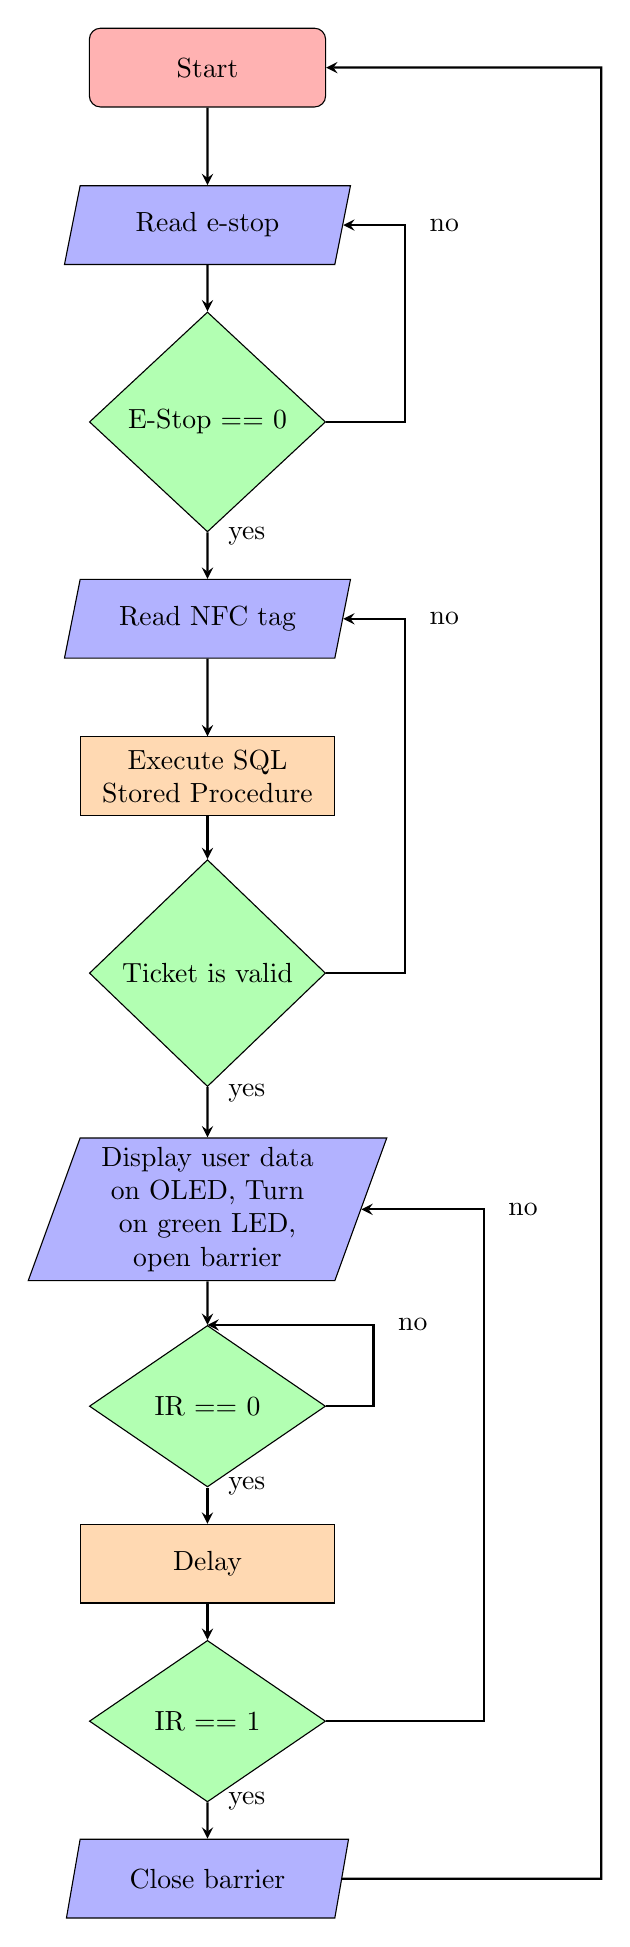
\begin{tikzpicture}[node distance=2cm]

\node (start) [startstop] {Start};
\node (in_estop) [io, below of=start] {Read e-stop};
\node (dec_estop) [decision, below of=in_estop, yshift=-0.5cm] {E-Stop == 0};

\node (nfc_read) [io, below of=dec_estop, yshift=-0.5cm] {Read NFC tag};

\node (sql_sp) [process, below of=nfc_read, xshift=0cm] {Execute SQL Stored Procedure};
\node (dec_nfc) [decision, below of=sql_sp, yshift=-0.5cm] {Ticket is valid};
\node (out1) [io, below of=dec_nfc, yshift=-1cm] {Display user data on OLED,
Turn on green LED,
open barrier};
\node (dec_ir_1) [decision, below of=out1, yshift=-0.5cm] {IR == 0};
\node (delay) [process, below of=dec_ir_1, xshift=0cm] {Delay};
\node (dec_ir_2) [decision, below of=delay] {IR == 1};
\node (out_2) [io, below of=dec_ir_2] {Close barrier};

\draw [arrow] (start) -- (in_estop);
\draw [arrow] (in_estop) -- (dec_estop);
\draw [arrow] (dec_estop.east) -| ++(1,0) |- node[xshift=5mm] {no} (in_estop.east);
\draw [arrow] (dec_estop) -- node[anchor=south,xshift=5mm] {yes} (nfc_read);
\draw [arrow] (nfc_read) -- (sql_sp);
\draw [arrow] (sql_sp) -- (dec_nfc);
\draw [arrow] (dec_nfc.east) -| ++(1,0) |- node[xshift=5mm] {no} (nfc_read);
\draw [arrow] (dec_nfc) -- node[anchor=south,xshift=5mm] {yes} (out1);
\draw [arrow] (out1) -- (dec_ir_1);
\draw [arrow] (dec_ir_1.east) -| ++(0.6,0) |- node[xshift=5mm] {no} (dec_ir_1.north);
\draw [arrow] (dec_ir_1) -- node[anchor=south,xshift=5mm] {yes} (delay);

\draw [arrow] (delay) -- (dec_ir_2);

\draw [arrow] (dec_ir_2.east) -| ++(2,0) |- node[xshift=5mm] {no} (out1);
\draw [arrow] (dec_ir_2) -- node[anchor=south,xshift=5mm] {yes} (out_2);
\draw [arrow] (out_2) -- ++(5,0) |- (start);

\end{tikzpicture}
\end{document}
